There has been a fundamental paradigm shift in the landscape of how we build software over the last 2 decades.
Originally, the compute stack was envisaged with the assumption that a single program would run on a single machine.
In this traditional model, system software abstractions subsumed the management of resources for processor, memory, disk and physically connected peripherals within the context of the machine.
However, this landscape rapidly changed with the evolution toward software being served on the backbone provided by the internet.
Now, an `application' is realized through the cooperation of multiple distinct sub-applications (services) running collaboratively.
For example a single application my contain one or more self-contained database, memcache, logging, application logic, and AI model applications interfacing each other over APIs as shown in Figure~\ref{fig:intro} (left).
We call these applications \emph{diffuse applications}.


This work contends that the fundamental programming paradigms in computing has not evolved at pace.
The abstractions envisioned during the era of the single machine computational model is still present at the programming interface and throughout the runtime stack leading to significant and costly complexity.


To address this complexity, two keystone abstractions have recently emerged to facilitate the development of these diffuse applications.
The first of these abstractions is the introduction and rapid dissemination of containerization service platforms.
With what started as a key insight articulated in ``The Datacenter as a Computer,'' Google would innovate their Borg system and ultimately released it open source as Kubernetes.
With Kubernetes, the underlying hardware resources would be abstracted away with the introduction of \emph{pods} (virtual machines), and other resources that can be virtually networked together and otherwise configured irrespective of the physical hardware.
Today, Kubernetes is the most prevalent containerized service abstraction layer in cloud computing.
The second of keystone abstraction would be coined ``Severless Computing'' and gained prominence with the introduction of Amazons Lamda functions.
This FaaS abstraction would facilitate the development of diffuse applications at the level of functions and abstract away the underlying containerized service ecosystem.
A programer can simply make function calls in their favorite language without every needing to be aware of where the function will run nor the system level resources that would be allocated or managed.

\begin{figure}[tb]
    \centering
    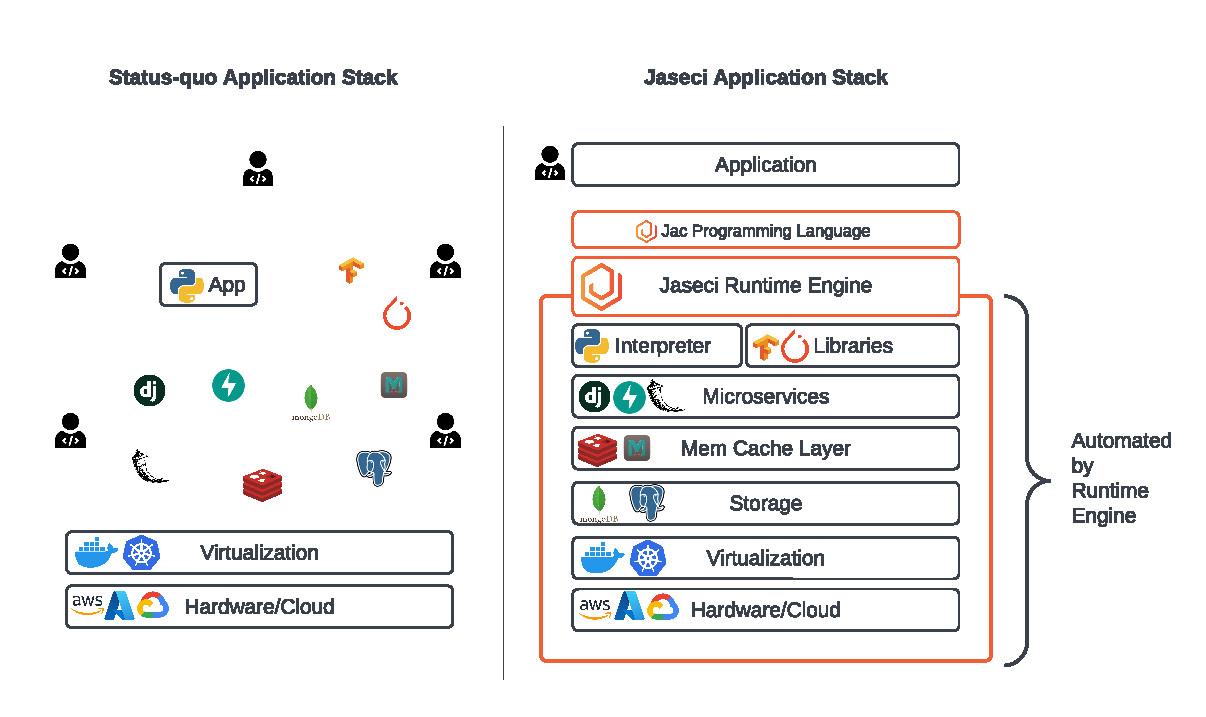
\includegraphics[width=\linewidth]{figures/jaseci_stack.pdf}
    \caption{Comparison between status quo development of production grade \emph{diffuse} applications (left), and the Jaseci technology stack that hides and automates an expanded set of subsystems through raising the level of abstraction (right).}
    \label{fig:intro}
\end{figure}



Though these two abstractions have been highly impactful, these innovations in our stack architecture represent a bottom up evolution of abstractions.
As a result, programmers are still left with single-machine abstractions at the programming interface and must grapple with a significant amount of complexity.
For example, traditional languages and their runtime stacks are predominately designed with the goal of hiding and managing intra-machine resources while what is needed for diffuse applications is the hiding and management of inter-machine resources.
Analogous to the virtualization and management of allocated memory on the heap provided by garbage collectors in modern languages (intra-machine), the virtualization and management of resources such as microservice creation, scheduling and orchestration alongside policies for organizing distributed databases, mem caches, logging and other highly complex subsystems (inter-machine) is not only needed, but as we show in this work, possible and practical.
Without this raising of the level of abstraction, it has become prohibitively difficult for a single engineer to invent, build, deploy, launch, and scale modern cutting edge applications.

To the best of our knowledge, we are not aware of a thorough, wholistic, and top-down design of a serverless programming paradigm and computational stack from the language level down through the system runtime stack to hide this expanded set of resources.

In this work, we present a wholistic design approach with the goal of abstracting away and automating a new class of underlying systems, allowing a programmer to articulate solutions and diffuse applications at the problem level.
We present the design of a \emph{diffuse runtime execution engine} we call \textbf{Jaseci}, and a \emph{data-spacial programming language} we call \textbf{Jac}.

The design of Jaseci and Jac has initially been inspired to by sophisticated emerging AI applications at scale and is driven by two key insightss.

\begin{itemize}

    \item \emph{Higher level abstractions are needed at the language level to allow single creators to work at the problem level to build end-to-end diffuse AI products.}
    \item \emph{A new set of abstractions across the language runtime and system stack is needed to automate and hide the class of inter-machine resources from the programmer.}

\end{itemize}

\noindent
To this end we present techniques across two categories,

\begin{enumerate}


    \item \emph{Jac Language} - A language that introduces a new set of abstractions, namely \textbf{data-spacial scoping} and \textbf{agent oriented programming}. These abstractions natively facilitates the emerging need to reason about and solve problems with graph representations as well as the need for algorithmic modularity and encapsulation to hide a new class of inter-machine resources.
    \item \emph{Jaseci Diffuse Runtime Engine} - A runtime that raises the abstraction layer to the problem solving level where the runtime engine subsumes responsibility for not only for the optimization of program code, but the orchestration, configuration, and optimization of the full cloud compute stack and inter-machine resources (such tasks as container formation, scaling and optimization).


\end{enumerate}


Jaseci and Jac is fully functional, open-source~\cite{jaseci-website,jaseci-github,jaseci-pypi}, and used in production for four real-world products today.
These commercial products were built entirely on the Jaseci staci and includes Myca~\cite{myca-website}, HomeLendingPal~\cite{hlp-website},  ZeroShotBot~\cite{zsb-website} and TrueSelph~\cite{ts-website}.
Across these and other projects, the Jac language has been used by dozens of programmers in the creation of production software and Jaseci deployments support tens of thousands of production queries per day currently.
In practice, our initial infrastructure has been leveraged in practice to achieve 10x reduction in development time and near 100\% elimination of typical backend code needed for a complicated AI based application.

The specific contributions of this paper include:
\begin{itemize}
    \item We formulate the problem of development complexity and present a top down programing paradigm and runtime stack for diffuse applications.
    \item We describe the design and implementation Jaseci's \textbf{diffuse runtime execution engine}.
    \item We introduce Jac, a language that implements a \textbf{data-spacial} programming paradigm (the first of its kind).
    \item We describe the utility of Jaseci and Jac through real world case studies of building out a real production scale-out product.
\end{itemize}

We find that the wholistic design philosophy and resulting paradigm of Jaseci and Jac is a promising one.
Multiple development teams have adopted the data spacial programming model of Jac and the diffuse runtime execution engine in Jaseci to build sophisticated AI products with significantly reduced complexity and teaming.